\documentclass[12pt,twoside,final]{book}

%\usepackage[portuges,brazil]{babel}
\usepackage[latin1]{inputenc}

\usepackage{indentfirst}
\usepackage{ae}
\usepackage{harvard}
\usepackage{amssymb,fancyhdr,fancybox,epsfig,psfrag,amsmath,tabularx}
\usepackage[paperwidth=8.5in,paperheight=11in,hmargin={25mm,20mm},vmargin={20mm,20mm}]{geometry} %tamanho letter

%Packages added by me
\usepackage{appendix}

\usepackage[color]{showkeys}
\definecolor{refkey}{rgb}{0.39,0.58,1}
\definecolor{labeled}{rgb}{1,0,0}
\usepackage[Lenny]{fncychap}
\setlength{\headheight}{15pt}

%=========================================== Headers =========================================

\renewcommand{\chaptermark}[1]{\markboth{\chaptername\ \thechapter. \ #1}{ }}
\renewcommand{\sectionmark}[1]{\markright{\thesection. \ #1}}
\fancyhead{}
\fancyfoot{}
\fancyhead[LE,RO]{\thepage}
\fancyhead[RE]{\nouppercase{\leftmark}}
\fancyhead[LO]{\nouppercase{\rightmark}}
%==============================================================================================


\input{macros}

\begin{document}

\pagenumbering{roman}
\pagestyle{plain}

%Tese em portugu�s
%================================================================================================
%================================= PRIMEIRA FOLHA INTERNA  ======================================
%================================================================================================

%\thispagestyle{empty} %Tirando o numero da primeira p�gina
\includegraphics [width=2cm] {unicamp.eps}

\vspace*{2.0cm}

\begin{center}
\large TIAGO DE FREITAS PEREIRA
\end{center}

\vspace*{3cm}

\begin{center}
{\sc ``A COMPARATIVE STUDY OF COUNTERMEASURES TO DETECT SPOOFING ATTACKS IN FACE AUTHENTICATION SYSTEMS"}
\\[1in]
{\sc ``UM ESTUDO COMPARATIVO DE CONTRAMEDIDAS PARA DETECTAR ATAQUES DE SPOOFING EM SISTEMAS DE AUTENTICA��O DE  FACES"}
\end{center}

\vspace*{3.25cm}

\null \vfill

\begin{center}
CAMPINAS\\2013
\end{center}



% parte de tr�s da primeira folha interna fica em branco
\newpage
\null \vfill
\thispagestyle{empty} %Tirando o numero da primeira p�gina
\newpage
\addtocounter{page}{-1}
%================================================================================================
%====================================== FOLHA DE ROSTO ==========================================
%================================================================================================
\includegraphics [width=2cm] {unicamp.eps}

\begin{flushleft}
\large \hspace*{2.5cm} UNIVERSIDADE ESTADUAL DE CAMPINAS\\
          \hspace*{2.5cm} Faculdade de Engenharia El�trica e de Computa��o
\end{flushleft}

\vspace*{1cm}
\begin{center}
\large TIAGO DE FREITAS PEREIRA
\end{center}

\vspace*{0.5cm}

\begin{center}
{\sc ``A COMPARATIVE STUDY OF COUNTERMEASURES TO DETECT SPOOFING ATTACKS IN FACE AUTHENTICATION SYSTEMS"}
\\[0.5in]
{\sc ``UM ESTUDO COMPARATIVO DE CONTRAMEDIDAS PARA DETECTAR ATAQUES DE SPOOFING EM SISTEMAS DE AUTENTICA��O DE FACES"}


\end{center}

\vspace*{0.5cm}

\begin{flushright}
\begin{minipage}{9.0cm}

Masters dissertation presented at the School of Electrical and Computer Engineering in partial fulfillment of the requirements for masters degree in Electrical Engineering. Concentration Area: Computer Engineering 
\\[0.2in]
Disserta��o de Mestrado apresentada na Faculdade de Engenharia El�trica e de Computa��o como  parte dos
requisitos exigidos para a obten��o do t�tulo de Mestre em Engenharia El�trica. �rea de
concentra��o: Engenharia de Computa��o

\end{minipage}
\end{flushright}

\null \vfill
\begin{minipage}{15cm}
Orientador: Prof. Dr. JOS� MARIO DE MARTINO
\vspace*{0.7cm}
\end{minipage}

\begin{minipage}{7cm}
\small
Este exemplar corresponde a vers�o final da disserta��o de mestrado apresentado pelo
aluno, e orientado pelo Prof. Dr. Jos� Mario De Martino\\[4mm]
\rule{7.0cm}{0.2mm} \hfill
\end{minipage}

\vspace*{0.5cm}

\begin{center}
CAMPINAS\\2013
\end{center}


%%%%%
%NEW BLANK PAGE
\newpage
\null \vfill
\thispagestyle{empty} %Tirando o numero da primeira p�gina
\addtocounter{page}{-1}


\newpage
%FICHA CATALOGRAFICA
%\includepdf[pages=-,pagecommand=\thispagestyle{plain} ,scale=1]{docs/Ficha-Catalografica-Protocolo-1355789.pdf}
\includepdf[scale=1.09]{docs/Ficha-Catalografica-Protocolo-1355789.pdf}


%\newpage
%comissao julgadora
\includepdf[pages=-,pagecommand=\thispagestyle{plain}]{docs/julgamento.pdf}

\newpage %verso em branco
\thispagestyle{empty} %Tirando o numero da primeira p�gina
\addtocounter{page}{-1}
\null
\newpage


%Tese em portugu�s e ingl�s
%%================================================================================================
%================================= PRIMEIRA FOLHA INTERNA  ======================================
%================================================================================================
\vspace*{2.0cm}
\begin{center}
\large Fulano de Tal
\end{center}


\vspace*{4.8cm}

\begin{center}
{\sc \Large  Coloque aqui o t�tulo da tese; Coloque aqui o t�tulo \\ da tese;
Coloque aqui o t�tulo da tese;  Coloque aqui }
\end{center}

\vspace*{1cm}
\begin{center}
{\sc \Large  Place here the thesis' title;Place here the thesis'\\ title; Place here the thesis' title ;
Place here }
\end{center}

\vspace*{3.25cm}


\null \vfill

\begin{center}
Campinas\\2012
\end{center}
\newpage
% parte de tr�s da primeira folha interna fica em branco

\null \vfill
\newpage


%================================================================================================
%====================================== FOLHA DE ROSTO ==========================================
%================================================================================================

\begin{center}
\large Universidade Estadual de Campinas\\
Faculdade de Engenharia El�trica e de Computa��o
\end{center}

\vspace*{1.0cm}
\begin{center}
\large Fulano de Tal
\end{center}


\vspace*{1.3cm}

\begin{center}
{\sc  Coloque aqui o t�tulo da tese; Coloque aqui o t�tulo da tese;  \\ 
Coloque aqui o t�tulo da tese;  Coloque aqui o t�tulo da tese;}
\end{center}

\vspace*{0.5cm}

\begin{center}
{\sc   Place here the thesis' title;Place here the thesis'\\ title; Place here the thesis' title ;
Place here }
\end{center}

\vspace*{1.0cm}

\begin{flushright}
\begin{minipage}{11.0cm}
Tese de doutorado apresentada � Faculdade de Engenharia El�trica e de Computa��o como  parte dos
requisitos exigidos para a obten��o do t�tulo de Doutor em Engenharia El�trica. �rea de
concentra��o: Automa��o. 

\vspace*{0.5cm}

Doctorate thesis presented to the School of Electrical and Computer Engineering
in partial fulfillment of the requirements for the degree of Doctor in Electrical
Engineering. Concentration area: Automation

\vspace*{1.0cm}
Orientador (Tutor): Prof. Dr. Pedro Luis Dias Peres

\end{minipage}
\end{flushright}

\null \vfill
\begin{minipage}{7cm}
\small
Este exemplar corresponde � vers�o final da tese defendida pelo
aluno, e orientada pelo Prof. Dr. Pedro Luis Dias Peres\\[4mm]
\rule{7.0cm}{0.2mm} \hfill 
\end{minipage}

\begin{center}
Campinas\\2012
\end{center}

%================================================================================================
%============================== Ficha (Somente na vers�o final) =================================
%================================================================================================
\newpage

\begin{center}
\vspace*{10cm}
Insira nesta p�gina a sua ficha catalogr�fica (somente vers�o final). Obs. � conveniente
converter o documento fornecido pela BAE (normalmente .doc) em um arquivo .ps. Para a vers�o
preliminar da tese (antes da defesa), simplesmente remova essa p�gina.
\end{center}
% Observa��o: a ficha fornecida pela BAE normalmente � fornecida em formato .doc. Existem diversas
% maneiras de converter .doc em .ps. 

% Descomente as duas pr�ximas linhas (e comente acima desde o begin{center} at� o end{center}) para inserir a ficha catalogr�fica caso a mesma j�  tenha sido convertida para .ps (no caso ficha.ps)

%\epsfxsize=0.925\columnwidth
%\epsffile{ficha.ps}

\null \vfill
\newpage

%================================================================================================
%============================== Folha de aprova��o (Somente na vers�o final) ====================
%================================================================================================


\begin{center}
\vspace*{10cm}
Insira nesta p�gina a folha de aprova��o fornecida pelo seu programa de p�s-gradua��o (somente vers�o final). 
Obs. � conveniente scanear o documento e convert�-lo para o formato .ps. Para a vers�o
preliminar da tese (antes da defesa), simplesmente remova essa p�gina.
\end{center}

% Escanear a folha de aprova��o fornecida pela CPG e converter para .ps ou .eps. A id�ia
% � inserir como uma figura. � muito prov�vel que ser� necess�rio fazer ajustes no
% tamanho, mexendo no comando \epsfxsize

% Descomente as duas pr�ximas linhas (e comente acima desde o \begin{center} at� o \end{center})
%\epsfxsize=0.985\columnwidth
%\hspace*{-1.25cm}\epsffile{aprov.eps}

\null \vfill
\newpage
% verso da folha de aprova��o em branco
\null \vfill
\newpage


%======================================== Dedicat�ria =========================================
\null\vfill
\begin{flushright}
\begin{minipage}{6.5cm}
{\sc 
To my parents \\

To my fianc\'ee Carolina Scarton}
\end{minipage} \\[8mm]
\end{flushright}
\newpage %verso em branco

\null
%==============================================================================================


%======================================= Agradecimentos =======================================
\chapter*{Acknowledgment}

%\noindent Text \\[2mm]

\noindent More than two years were necessary to finish this work and many people got involved. \\

First of all, I would like to thank Prof. Dr. Jos\'e Mario De Martino for his guidance, incentive, friendship and patience in this journey. \\

Many thanks to Dr. S\'ebastien Marcel, Dr. Andr\'e Anjos and Ivana Chingovska, from the IDIAP Research Institute. Their supervision in the four months in Switzerland were definitely decisive to complete this masters dissertation. A special thanks to Dr. Andr\'e Anjos for his guidance, friendship and the doses of cacha\c{c}a. I also would like to thank Dr. Manuel G{\"u}nter, Dr. Elie El Khoury, Dr. Nesli Erdogmus, Laurent El Shafey and Jukka Komulainen (University of Oulu) for their support and fellowship. \\

Thanks to CPqD, for encourage me in this project, releasing so many hours of work and for fund part of this research. A special thanks to Norberto Alves Ferreira, Claudinei Martins, Eliana De Martino, Emilio Nakamura, Marcus de Assis Angeloni, Jos\'e Eduardo de Carvalho Silva, Ricardo Violatto, Mario Uliani and the big master Flavio Sim\~oes. \\

Thanks to my friends Geovane Shimizu, Bruno Cafeo and Diego Silva for just being there. \\

Thanks to my parents Antonio Alberto (Tote) and Sueli, and brother Rodrigo for the unconditional love and support, even don't understanding a bit what I am doing. A special thanks to my grandma Christina. She was a great example of a teacher and also my first one. \\

A very special thanks to my best friend and fianc\'ee Carolina Scarton, for her support, care, patience and unconditional love during all these years.


\newpage %verso em branco

\null

%==============================================================================================


%======================================== Frase Miss Brasil ===================================
\newpage
\null\vfill
\begin{flushright}
\begin{minipage}{9.0cm}

%If you have nothing better to say, is better to shut up.
Two things are infinite: the universe and human stupidity; and I'm not sure about the universe. 

\end{minipage}
\end{flushright}


\begin{flushright}
Albert Einstein
\end{flushright}

\newpage %verso em branco

\null
%==============================================================================================



\baselineskip 1.1 \baselineskip

%================================= Resumo e Abstract ========================================
\chapter*{Resumo}


\begin{quotation}
\noindent Resumo

\vspace*{0.5cm}

\noindent Palavras-chave: 
\end{quotation}


\newpage
\null



\chapter*{Abstract}


\begin{quotation}


\noindent Abstract

\vspace*{0.5cm}

\noindent Key-words: 
\newpage% verso em branco
\end{quotation}

\newpage
\null




%=============================== lista de tabelas e figuras ==========================
\listoffigures
\newpage


\listoftables
\newpage



%============================ acr�nimos, s�mbolos e nota��es ========================
%============================Acronimos e Notacao=================================================
\chapter*{Lista de Acr�nimos e Nota��o}
\begin{tabular}{ll}
$AUC$ & \textit{Area Under the Curve} \\
$DoG$ & \textit{Difference of Gaussians} \\
$EER$  & \textit{Equal Error Rate} \\ 
$FAR$  & \textit{False Acceptance Rate} \\
$FRR$ & \textit{False Rejection Rate} \\
$GLCM$ & \textit{Gray Level Co-occurrence Matrix} \\
$HMM$ & {Hidden Markov Model} \\
$HTER$ & \textit{Half Total Error Rate} \\
$LBP$ & \textit{Local Binary Patterns} \\
$LBP-TOP$ & \textit{Local Binary Patterns from Three Orthogonal Planes} \\
$MLP$ & \textit{Multi Layer Perceptron} \\
$PLS$ & \textit{Partial Least Square} \\
$ROC$ & \textit{Receiver Operating Characteristics} \\
$SVM$ & \textit{Support Vector Machines} \\
\end{tabular}


\newpage
% verso em branco (sem numeracao na pagina).

%==============================================================================================


%=============================== sum�rio =============================================
\tableofcontents


\newpage
%caso o sum�rio acabe em uma p�gina �mpar, o verso ser� em branco
\null \vfill
\newpage

%Agora muda para o estilo fancy
\pagestyle{fancy}

%%%%%%
% CRIAR FINAL REMARKS
%%%%%%%%


\chapter{Introduction}
\label{chap:introduction}

In a modern society, the authentication procedure is an important task to protect data and resources (physical or digital). Consisting of a confirmation of a claimed identity, the authentication procedure is the first and most critical task of security step, restricting access to unauthorized users. 

Biometrics is the science of recognizing the identity of a person based on their physical attributes and / or behavior, such as face, fingerprints, hand veins, voice or iris \cite{li2011handbook}. The use of biometrics in an authentication procedure has some advantages. Naturally, is not possible to forget or transfer a biometric trait and it hardly disappears (perhaps only in case of a seriously accidents). However, biometrics has some drawbacks. Compared with regular authentication systems, such as passwords or tokens, which are precise, biometric authentication systems have probabilistic behavior. It turns out that biometrics hardly has perfect match; therefore, authentication systems have to deal with error rates. These errors rates can vary depending on a number of factors. As an example, our voice can vary drastically  when we get sick or when we are under stress and this impacts a speaker authentication system. Aging, illumination, pose and face expressions are classical issues in face authentication systems.


The use of biometrics in our daily lives has grown in the last decade and we can quote several examples of this. The confirmation of an identity in the brazilian electoral process is based on fingerprints. In Brazil, a bank replaced the use of passwords to palm vein authentication in ATMs. The demand for security pushes the market to biometrics. A recent marked research estimates that the overall market for voice and face biometrics is expected to reach nearly US\$3 billions by the end of 2018\footnote{\url{http://www.biometricupdate.com/201307/voice-biometrics-and-how-far-weve-come/?goback=\%2Egde\_40210\_member\_258411747}}.


A biometric authentication system can be represented with the simple flow chart in Figure \ref{fig:diagram_attacks}.

\begin{figure}[!htb]
\begin{center}
\includegraphics [width=14cm] {images/diagram_attacks.pdf}
\caption[Simple architecture of a regular biometric authentication system]{Simple architecture of a regular biometric authentication system (adapted from \cite{xiao2005security})} \label{fig:diagram_attacks}
\end{center}
\end{figure}

Firstly, the biometric trait is captured using a some kind of sensor. Secondly, the captured biometric trait is processed in order to extract the biometric features. When it is in an enrollment procedure, these features will generate a biometric reference, and it will be stored in a database. In an authentication procedure, these features will be compared with the stored biometric reference. It is possible to observe, in the same Figure, that attacks can be done at any point of the architecture \cite{xiao2005security}. 
%The next subsections discuss each one of the possible points of attack and how to mitigate it.

%\subsection{Replay attack}
%\label{sec:rep}

The \textbf{replay attack} is performed by injecting a biometric data previously sent, of the target identity, in order to have a non authorized access. This data can be obtained sniffing the biometric authentication software. To mitigate this kind of attack, the biometric system should ensure that the provided data was not injected artificially \cite{xiao2005security}. A common way to protect against this kind of attack, is to associate a timestamp to the data. As it is improbable to have exactly the same biometric data in different times, this method can be quite effective.

%\subsection{Biometric reference attack}

The \textbf{biometric reference attack} is performed where the biometrics are stored. This kind of attack, include actions such as the inclusion, removing, modifying and steal biometric references. Among this actions, the possibility to steal a biometric reference is the most dangerous threat, since it is possible to work in a reverse engineering process to regenerate the biometric trait. 

Using a hill climbing technique to optimize to the position and the orientation of the minutia \cite{MartinezDiaz2006} and \cite{hill2001risk} shown that is possible to generate synthetic fingerprints compatible with fingerprints stored in a database. Fake fingers (with a real fingerprint) with gummy or silicone can be generated with this minutia. It is possible also to inject these minutia in the \textbf{Processing} module (see Figure \ref{fig:diagram_attacks}) in order to deceive the authentication system. 

To mitigate the risk of this kind of attack, best practices in security recommends to encrypt the biometric references and to increase the policy to access these biometric references. 

%\subsection{Man-in-the-middle}

In the \textbf{man in the middle attack}, the biometric data is intercepted in any point of the architecture in Figure \ref{fig:diagram_attacks}.  As shown in the Figure \ref{fig:diagram_attacks}, the attacker can:
\begin{itemize}
        \item Manipulate the matching score;
        \item Manipulate the biometric authentication response;
        \item Steal biometric data;
        \item Inject biometric data (as shown in the replay attack).
\end{itemize}

The same security recommendations aforementioned to deal with this security breaks can be used here; i.e. encrypt the data before transmission, increase the security grants and so on. 

%\subsection{Ataque de Spoofing}

The \textbf{spoofing attack}, in biometric systems, is a direct attack to the biometric sensor; i.e. a forged biometric trait is presented to the biometric sensor in order to deceived it. The goal is to pretend to be someone else in order to get forbidden privileges. Most of biometric systems can be spoofed. Next subsections presents a brief discussion about spoofing in different biometric traits:

\subsubsection{Fingerprint}

In fingerprints verification systems, the attacker can forge a fingerprint with different materials (gummy, silicone, etc). \cite{matsumoto2002impact} and \cite{leyden2002gummi} discusses how to generate fake fingerprints using materials easily found in supermarkets. Figure \ref{fig:finger_attack} shows how easy is to create a molds from a live fingers and to reproduce its fingerprints with gummy. This fake fingers can be used  to spoof a fingerprint biometric systems.

\begin{figure}[!htb]
\begin{center}
\includegraphics [width=16cm] {images/finger_print_attack.pdf}
\caption[Creating a fake fingerprint]{Creating a fake fingerprint (Adapted from \cite{matsumoto2002impact})} \label{fig:finger_attack}
\end{center}
\end{figure}

Recently in Brazil (2013), was reported that doctors in S\~ao Paulo were arrested after being caught in the act of using fake fingers made of silicone and imprinted with real fingerprints to defraud a hospital's biometric punch-in clock\footnote{\url{http://www.foxnews.com/us/2013/03/13/brazilian-doctors-use-fake-silicone-fingers-to-defraud-hospital-punch-in-clock/}}.

A more sophisticated attack is discussed in \cite{MartinezDiaz2006} and \cite{hill2001risk}. These papers use a hill climbing technique to optimize  the position and the orientation of the minutia. With this optimization was possible to generate fingerprints compatible for match.

%Using a hill climbing technique to optimize to the position and the orientation of the minutia  shown that is possible to generate fingerprints compatible with fingerpri
%A more sophisticated attack were discussed in \cite{uludag2004attacks}. This paper uses a hill climbing procedure to optimize the position and the orientation of the minutia in a minutia based fingerprint verification system. The optimized result of the minutia can be used to generate a fake finger.

%FALAR DOS SENSORES.

%http://www.tabularasa-euproject.org/news/selected-news-related-to-spoofing-attacks

\subsubsection{Speaker}

For speech biometrics, the attacker can forge a human voice by mimicry or recording the voice of the target identity and replaying back to the microphone. 

\cite{chetty2004liveness} and \cite{eveno2005speaker} address the problem using audio-visual features. The first one proposes a bi-modal authentication system using the face information in order to increase security. The second one correlates the lip movements with the content of the speech as a security barrier.

\cite{QimingZhu} analyse the speech signal itself applying the 1-dimensional $LBP$ (Local Binary Pattern) followed by a SVM (Support Vector Machines) in order to detect spoofs.

\subsubsection{Iris}

Iris biometrics has been traditionally regarded as one of the most reliable and accurate biometric traits, but as the other biometric traits it can also be spoofed. A simple way to spoof an iris recognition system is using a high quality printed image. More sophisticated attacks using contact lenses can also be carried out.

Countermeasures to deal with this kind of attacks can be deployed in hardware (with a specific equipment) or in the software \cite{Galbally_ICB-2012}. Especially in the software level, \cite{Galbally_ICB-2012} addresses the problem using various type of features, including a set of  high pass filters, motion features and occlusion filters in the iris images followed by a binary classifier as countermeasure. 

An approach based on textures was carried out by \cite{ZhuoshiWei}. This countermeasure uses the co-occurrence matrix descriptor followed by a binary classifier.

%Measuring the pupil reflex using a set of high filters, \cite{kanematsu2007highly}
% \cite{johnson2010multimodal}, \cite{kanematsu2007highly} and \cite{pacut2006aliveness} are works addressing spoofing attacks in iris biometric system. 

\subsubsection{Face}

Recently, the media has reported some situations of attacks in deployed face recognition systems. Using simple photographs, a research group from University of Hanoi showed how easy is to spoof the face authentication systems deployed in Lenovo, Asus and Toshiba Laptops \cite{BlackHat2009}. Since the release \textit{Ice Cream Sandwich}, the Android OS come with a built-in face authentication system to unlock the mobile phone. Since then, it has been extensively demonstrated around the web how easy it is to spoof this face recognition system\footnote{\url{http://www.itproportal.com/2011/11/14/ice-cream-sandwich-facial-recognition-cracked/}}. As a consequence, an eye blinking detection has been introduced in the most recent version of the Android OS. Spoofing in face authentication will be discussed in details in the Chapter \ref{chap:Spoofing}. \\ \\ 

Several technologies related to information security can be deployed in a biometric authentication systems in order to mitigate the mentioned attacks. We can highlight:
\begin{itemize}
        \item Encrypt the biometric data;
        \item Improve the security policies;
        \item Convey the biometric data using a secure channel;
        \item Deploy all modules of the architecture in a physical arrangement that cannot be penetrated;
        \item Using more than one authentication factor.
\end{itemize}
However, in a spoofing attack, the target is the biometric sensor, and in the architecture presented in Figure \ref{fig:diagram_attacks}, is not possible to apply any of the security tools to prevent this kind of attack, becoming the most fragile point. To mitigate this kind of vulnerability, effective countermeasures against face spoofing have to be deployed.


\section{Scope and Contributions}
\label{sec:scope}

Focusing in antispoofing countermeasures for face authentication, the goal of this masters dissertation is two fold. The first one, we introduce a novel method to detect face spoofing using the spatiotemporal (dynamic texture) extensions of the Local Binary Pattern. The key idea of the approach is to learn and detect the structure and the dynamics of the facial micro-textures that characterise real faces but not fake ones. The second one, is to provide a comparative study of the state of the art countermeasures for face antispoofing. The key contribution of this comparative study is to covers tests in all video face antispoofing databases freely available focusing in the biases that these databases can introduce in the countermeasures.

\section{Organization of the Thesis}
\label{sec:scope}

Besides this introduction, that presented the motivation of this work, the dissertation has four more chapters. 

The Chapter \ref{chap:Spoofing} defines spoofing attacks in face authentication, presenting the main countermeasures and the resources available for this research.

The Chapter \ref{chap:Proposed_Countermeasures} defines and presents the results of the proposed countermeasure based on dynamic texture, the first contribution of this dissertation and their results.

The Chapter \ref{chap:Comparative_Study} defines and presents the results of the comparative study of face antispoofing countermeasures.

Finally the Chapter \ref{chap:Conclusions} presents the conclusions and the future work.

\chapter{Biometrics}
\label{chap:Biometrics}

Some text.

\section{Introduction to Biometric Systems}
\label{sec:IntroBiome}

Biometrics is the science of recognizing the identity of a person based on their physical attributes and / or behavior, such as face, fingerprints, hand veins, voice or iris \cite{li2011handbook}. The use of biometrics as authentication factor has some advantages. Naturally, is not possible to forget or transfer a biometric trait and it hardly disappears (perhaps in case of a seriously accidents). Biometrics has some disadvantages. As an example, our voice vary drastically  when we get sick or when we are under stress. Unfortunately our facial trait change when we get old. It is important to remark that authentication based on biometrics is probabilistic, which means that errors can happen (????).

To use a biometric trait in a biometric system, the candidate train must satisfy the following requiriments.

\begin{itemize}
        \item Universality (every person must have it);
        \item Uniqueness (must distinguish people);
        \item Stability (must be stable along the time);
        \item Coletability (must be measure);
        \item Performance;
        \item Acceptance;
        \item Circunvention (low risk of frauds).
\end{itemize}


Table \ref{tb:comparacao} shows a comparative between the most used biometric traits \cite{maltoni2009handbook}. It can be observed that none of the presented biometric traits fulfil all the listed requirements and the selection of a trait depends on the application (??????) \cite{jain1999biometrics}.

%A Tabela \ref{tb:comparacao} apresenta um comparativo realizado por \cite{maltoni2009handbook} entre as caracter�sticas biom�tricas mais utilizadas. � poss�vel observar que nenhuma das biometrias apresentadas consegue atender todos estes requisitos com excel�ncia e a escolha de qual utilizar deve levar em conta a natureza e as exig�ncias de cada aplica��o \cite{jain1999biometrics}.

\begin{table}[ht]
\caption[Comparison of the most used biometric traits]{Comparison of the most used biometric traits \cite{maltoni2009handbook}}
\begin{center}
    \begin{tabular}{ | c | c | c | c | c | c | c | c |}
    \hline
    \textbf{Biometric trait} & \rotatebox{90}{\textbf{Universality}} & \rotatebox{90}{\textbf{Uniqueness}} & \rotatebox{90}{\textbf{Stability}} & \rotatebox{90}{\textbf{Coletability}} & \rotatebox{90}{\textbf{Performance}} & \rotatebox{90}{\textbf{Acceptance}} & \rotatebox{90}{\textbf{Circunvention}} \\ \hline
    Face                             & High      & Low  & Medium & High     & Low  & High      & Low \\ \hline
    Fingerprint                  & Medium  &  High    & High      & Medium & High     & Medium  & Medium \\ \hline
    Hand geometry         & Medium  & Medium & Medium & High     & Medium & Medium  & Medium \\ \hline
    Palm vein                   & Medium  & Medium  & Medium & Medium & Medium & Medium & High \\ \hline
    Iris                               & High      & High       & High     & Medium & High     & Low  & High \\ \hline
    Signature                   & Low   & Low   & Low  & High     & Low  & High     & Low \\ \hline
    Voice                           & Medium  & Low   & Low  & Medium & Low  & High     & Low \\ \hline
    \end{tabular}
\end{center}
\label{tb:comparacao}
\end{table}




\section{Attacks in Biometric Systems}
\label{sec:AttacksBiometric}

Talk about spoofing.
%Colocar o conteudo geral de spoofing neste cap.

\chapter{Spoofing Attacks}
\label{chap:Spoofing}

As aforementioned, spoofing attacks in biometrics are direct attacks to the biometric sensor. Spoofing techniques vary from different biometrics. This chapter discusses the spoofing attacks in different biometric traits focusing in face recognition.

\section{Spoofing Attacks in Biometrics}
\label{sec:SpoofingAttacksBiometrics}

It is always possible to create a spoofing attack to a biometric system. This sections discusses the occurrences of spoofing attacks in different biometric systems.

%The spoofing attack in biometric system is a direct attack to the biometric sensor; a forged biometric is presented to the biometric sensor. The goal is to pretend to be someone else in order to get some forbidden privileges. Spoofing techniques vary from biometrics, just for the record: In fingerprints based systems the attacker can forge a fingerprint  with different materials (gummy, silicone, etc) in order spoof the system as can be observed in \cite{uludag2004attacks}, \cite{leyden2002gummi} e \cite{matsumoto2002impact}. \cite{johnson2010multimodal}, \cite{kanematsu2007highly} and \cite{pacut2006aliveness} are works addressing spoofing attacks in iris biometric system. Finally \cite{chetty2004liveness} e \cite{eveno2005speaker} address speaker based biometric systems.


\subsection{Fingerprint}

In fingerprints based systems the attacker can forge a fingerprint with different materials (gummy, silicone, etc) in order spoof the system as can be observed. \cite{matsumoto2002impact} and \cite{leyden2002gummi} discusses how to generate fake fingerprints using materials that is possible easily to find in a supermarket. Figure X shows how easy is to create a mold from a live finger and to reproduce its fingerprint with gummy. This fake fingers can be used  to spoof a fingerprint biometric systems.

Figure X.

Recently in Brazil (2013), was reported that doctors in Sao Paulo were arrested after being caught in the act of using fake fingers made of silicone and imprinted with real fingerprints to defraud a hospital's biometric punch-in clock\footnote{http://www.foxnews.com/us/2013/03/13/brazilian-doctors-use-fake-silicone-fingers-to-defraud-hospital-punch-in-clock/}.

A more sophisticated attack were discussed in \cite{uludag2004attacks}. This paper uses a hill climbing procedure to optimise the position and the orientation of the minutia in a minutia based fingerprint verification system. This optimized minutia can be used to generate a fake finger.

FALAR DOS SENSORES.

%http://www.tabularasa-euproject.org/news/selected-news-related-to-spoofing-attacks

\subsection{Speaker}

For the speech biometrics the attacker can forge a human voice by mimicry or recording the voice of the target identity and replaying back to the microphone. \cite{chetty2004liveness} e \cite{eveno2005speaker} address the problem using audio-visual features. The first one proposes a bi-modal authentication system using the face information in order to increase security. The second one correlates the lip movements with the content of the speech.

PAPER analyses the speech signal itself applying the 1D-LBP (Local Binary Pattern) followed by a SVM (Support Vector Machines) in order to detect spoofs.

\subsection{Iris}

 \cite{johnson2010multimodal}, \cite{kanematsu2007highly} and \cite{pacut2006aliveness} are works addressing spoofing attacks in iris biometric system. 


\section{Spoofing Attacks in Face Recognition}
\label{sec:SpoofingAttacksFaceRec}

Because of its natural and non-intrusive interaction, identity verification and recognition using facial information are among the most active and challenging areas in computer vision research. Despite the significant progress of face recognition technology in the recent decades, wide range of viewpoints, ageing of subjects and complex outdoor lighting are still research challenges. Advances in the area were extensively reported in \cite{flynn2008handbook} and \cite{li2011handbook}. 

It was not until very recently that the problem of spoofing attacks against face biometric system gained attention of the research community. This can be attested by the gradually increasing number of publicly available databases \cite{pan2007eyeblink,tan2010face,zhangface,ChingovskaBIOSIG2012}. Two contests were organized in the last two years. The first one it was the IJCB 2011 "competition on counter measures to 2D facial spoofing attacks" \cite{ChakkaIJCB2011} which was the first competition conducted for studying best practices for non-intrusive spoofing detection. More recently, the ICB 2013 organized the "2nd competition on counter measures to 2D facial spoofing attacks" ????.

In authentication systems based on face biometrics, spoofing attacks are usually perpetrated using photographs, videos or forged masks. While one can also use make-up or plastic surgery as mean of spoofing, photographs and videos are probably the most common sources of spoofing attacks. Moreover, due to the increasing popularity of social network websites (facebook, flickr, youtube, instagram and others), a great deal of multimedia content - especially videos and photographs - is available on the web that can be used to spoof a face authentication system. In order to mitigate the vulnerability of face authentication systems, effective countermeasures against face spoofing have to be deployed.

DEPENDENTE E INDEPENDENTE DA COLABORACAO.

\subsection{Presence of vitality (liveness)}

Presence of vitality or liveness detection consists of  search for features that only live faces can possess. The eye blinking is an activity that humans do constantly. A regular human blinks once every 2 or 4 seconds in order to maintain the eyes clean and wet. This frequency can vary in stress conditions and/or in a high concentration task. In that situations the interval can extend to $\sim 20$ seconds. However, does not matter in what condition, in some point the eye blink will occur. Following that fact, \cite{pan2007eyeblink} propose a countermeasure measuring the eye blinking using hidden markov (HMM ???) mapping the state of eyes open and closed. Experiments carried out using a database created by the authors and freely available for download\footnote{http://www.cs.zju.edu.cn/~gpan/database/db\_blink.html}, shown an accuracy of 95.7\% .


%Apoiado na hip�tese de que faces vivas apresentam padr�es de movimento em certas regi�es da face altamente descorrelacionados se comparados a ataques, \cite{kollreider2009non} desenvolveu uma heur�stica baseada em fluxo �tico para explorar tal caracter�stica. Como refer�ncia para a heur�stica foram selecionadas as regi�es do centro da face e das orelhas como pode ser observado na Figura \ref{img_kollreider}.

EULERIAN.

\subsection{Scene}




\subsection{Differences in image quality assessment}


\section{Face Spoofing Databases}
\label{sec:Databases}

Discuss permeability of the databases.


\chapter{Developed Countermeasures}
\label{chap:Proposed_Countermeasures}
\chapter{The Comparative Study}
\label{chap:Comparative_Study}

\section{Databases Permeability}
\label{sec:Databases_Permeability}

\section{Evaluation Protocol}
\label{sec:Evaluation_Protocol}

\subsection{Intra Database Test Protocol}
\subsection{Inter Database Test Protocol}
\subsection{Evaluation Metrics}
\chapter{Comparative Study of Face Antispoofing Countermeasures}
\label{chap:Comparative_Study}

This chapter presents the experimental results of this comparative study of face spoofing countermeasures. The countermeasures compared in this dissertation and how each hyper-parameter was set is discussed in Section \ref{sec:Evaluated_countermeasures}. The Section \ref{sec:Evaluation_Protocol} presents the evaluation protocol applied in this dissertation and section \ref{sec:Metrics} presents metrics used. The data evaluated in this dissertation and how this data was organized in the experiments are covered in Section \ref{sec:data}. In Section \ref{sec:Comparative_experiments} we report our experimental results. Finally, Section \ref{sec:Experiments_finalremarks} presents the final remarks of the chapter.

The content of this chapter was published in the International Conference on Biometrics (ICB 2013) with the paper entitled ``Can Face Antispoofing Countermeasures Work in a Real World Scenario?" \cite{FreitasPereira_ICB_2013}.

%The Section \ref{sec:Intra_test} presents the results applying the Intra-test protocol. Section \ref{sec:Inter_test} presents the results applying the Inter-test protocol. In the Section \ref{sec:combination} the combination of databases is explored to train each one of the presented countermeasures. In Section \ref{sec:framework} the Score Level Fusion based Framework is explored to train each countermeasure. Finally Section \ref{sec:Experiments_finalremarks} summarizes the experiments.


\section{Evaluated countermeasures}
\label{sec:Evaluated_countermeasures}

Our comparative study considers four countermeasures that do not depend on user collaboration. Representing the state of the art in the face antispoofing research, each countermeasure explores one of the main cues mentioned in the Section \ref{sec:countermeasures} (Presence of vitality, Scene characteristics, and Differences in image quality assessment). Next subsections present the details of each countermeasure and how the hyper-parameters of each one was set.

\subsection{Motion Correlation}

As presented in Section \ref{sec:scene_cues}, the Motion Correlation \citep{AnjosIJCB2011} countermeasure measures the correlation between the motion of the face and it background. The source code of this countermeasure is freely available\footnote{\url{https://pypi.python.org/pypi/antispoofing.motion/}} in order to allow the reproduction of the results. There are, basically, two hyper-parameters in this countermeasure. The first one, is the number of frames used to compute the 5 parameters (see Section \ref{sec:scene_cues}). The second one is the binary classifier.

As the authors suggested, twenty frames to compute the 5 parameters are sufficient for the algorithm to converge in their experiments. The classifier suggested in the paper was one based on Multi-layer Perceptron. This classifier has, basically, the number of hidden layers and the number neurons in each hidden layer as hyper-parameters. The authors suggested one hidden layer and five neurons in this hidden layer as good tradeoff between computational complexity and performance. We adopted the suggested hyper-parameters in our experiments.

\subsection{Textures with $LBP$}

Presented in Section \ref{sec:quality_assessment}, the countermeasure based on Textures with $LBP$ \citep{ChingovskaBIOSIG2012} and \citep{maatta2011face} explores the differences in texture properties between real accesses and attacks in single frames. The source code of this countermeasure is also freely available\footnote{\url{https://pypi.python.org/pypi/antispoofing.lbp/}} in order to allow the reproduction of the results.

There are, basically, three hyper-parameters in this countermeasure. The first one is the geometrically normalized face size. The authors suggested a face size of $64 \times 64$ pixels. The second one is the configuration of the $LBP$ texture descriptor. The $LBP$ itself has several hyper-parameters \citep{inen2011computer} and the authors of both papers explored only some of them. In this dissertation, we follow the setup suggested by \cite{ChingovskaBIOSIG2012} using the $LBP_{8,1}^{u2}$. Finally the last hyper-parameter is the binary classifier. The best classifier tested by \cite{ChingovskaBIOSIG2012} was the Support Vector Machines (SVM) using the Radial Basis Function (RBF). 
%For this classifier the parameter $C$ (the cost of the loss function) and the $\gamma$ parameter (the variance of the radial function) was set to $1$ and $0.1$ respectively.

\subsection{Dynamic Textures with $LBP-TOP$}

Presented in the Chapter \ref{chap:Proposed_Countermeasures} as one of our contributions, the countermeasure based on dynamic textures with $LBP-TOP$, explores the texture dynamics to detect attacks in a frame sequence. The source code of this countermeasure is freely available\footnote{\url{https://pypi.python.org/pypi/antispoofing.lbptop/}} in order to allow the reproduction of the results.

There are, basically, three hyper-parameters in this countermeasure. The first one is the geometrically normalized face size. In our previous experiments (see Chapter \ref{chap:Proposed_Countermeasures}) we worked with face sizes of $64 \times 64$ pixels and we will keep this in the next experiments. The second hyper-parameter is the configuration of the $LBP-TOP$ descriptor. As in the $LBP$, the $LBP-TOP$ descriptor itself has several hyper-parameters and most of them were extensively tuned in Chapter \ref{chap:Proposed_Countermeasures}. As a good tradeoff between computational complexity and performance, we selected the following configuration: $LBP-TOP^{u2}_{8,8,8,1,1,1}$ with a single resolution. The last hyper-parameter is the binary classifier. The evaluation method proposed in the Chapter \ref{chap:Proposed_Countermeasures} suggests the SVM classifier with RBF kernel.


\subsection{Eye blinks}

The eye blink countermeasure used in this dissertation, uses a similar technique applied in Motion Correlation countermeasure \citep{AnjosIJCB2011}. The difference is the accumulated motion $M_D$, (see Equation \ref{eq:motion}) is computed between the face region and the eyes region as can be observed in the Figure \ref{fig:eye_blink}. 

\begin{figure}[!btb]
\begin{center}
\includegraphics [width=10cm] {images/eye_blink.pdf}
\caption[Eye blink countermeasure scheme]{Eye blink countermeasure scheme. The eye blink is measured as a motion correlation between the eyes region and the face region.}
\label{fig:eye_blink}
\end{center}
\end{figure}


The eye blink score for each single frame $n$ in a frame sequence, is computed using the following equation:
\begin{equation}
S_n=   \frac{M_{D_{eye}}(n)}{M_{D_{face}}(n)} - ravg(\frac{M_{D_{eye}}}{M_{D_{face}}})(n)
\label{eq:score_blink}
\end{equation}
where the $ravg$ is the remainder average in a frame sequence until the frame $n$. Then remainder average is computed averaging the remainder $M_D$ until the frame $n$. 

The trigger of this countermeasure is the number of blinks. In this dissertation, we will test one, two and three blinks as a trigger of a real access. The source code of this countermeasure is also freely available\footnote{\url{https://github.com/bioidiap/antispoofing.eyeblink}}.


\section{Evaluation Protocol}
\label{sec:Evaluation_Protocol}

For this comparative study, we will evaluate the intra-database and the inter-database (or cross-database) generalization. For that, we developed two test protocols: the intra-test protocol and the inter-test protocol. 

The intra-test protocol evaluates the intra-database generalization. It consists in training, tuning and testing a countermeasure with the respectively training set, development set and test set of one database.

The inter-test protocol is a little bit more challenging, since it tests the inter-database generalization (or cross-database). It consists in training and tuning a countermeasure with the training set and development set of one database and test it with the test set of others databases. 


%Firstly, we study how the countermeasures, presented in Section \ref{sec:countermeasures}, will perform in a more realistic condition. This condition consists in training and tuning each one of the countermeasures with one face anti-spoofing database and testing with another one. To report the performance in such a scenario, two evaluation protocols were designed to work with the databases described in Section \ref{sec_replay}. These protocols are the "intra-test" protocol and the "inter-test" protocol.


%The inter-test protocol evaluates the countermeasure performance in a more realistic scenario, close to real usage conditions. It consists in training and tuning a countermeasure with the training set and development set of one database and test it with the test set of another one. With this protocol, it is possible to evaluate the performance and the generalization power of a countermeasure in a set of unseen types of attacks.


\section{Evaluation Metrics}
\label{sec:Metrics}

The final performance of each countermeasure using both evaluation protocols in the test set of each database is reported with the Half Total Error Rate ($HTER$): 

\begin{equation}
\label{eq:HTER}
HTER(D_2)=\frac{FAR(\tau(D_1),D_2)+ FRR(\tau(D_1),D_2)} {2} ,
\end{equation}
where $\tau(D_1)$ is the decision threshold, $D_n$ is the dataset, $FAR$ is the False Acceptance Rate in the database $D_2$ and $FRR$ is the False Rejection Rate in the database $D_2$. In this protocol, the value of $\tau(D_n)$ is estimated on the Equal Error Rate (EER) using the development set of the database $D_1$. 

In this equation, to measure the performance using the intra-database protocol, is necessary to consider $D_1 = D_2$. To measure the performance using the inter-database protocol, just consider $D_1 \neq D_2$.


\section{Evaluated data}
\label{sec:data}

As the Motion correlation, $LBP-TOP$ and the eye blink countermeasures need a frame sequence to work, the databases appropriate for this dissertation are the Replay Attack Database (Section \ref{sec_replay}) and CASIA FASD (Section \ref{sec_casia}).

As already mentioned in Section \ref{sec_replay} the Replay Attack Database has three non-overlapping partitions; the training, development and test set for respectively train, tune and test a countermeasure. To run the proposed protocols in this database, we will use the train set to train the four countermeasures; the development set will be used to estimate the value of $\tau(D_1)$. Finally the test set will be used to report the $HTER(D_2)$.

The CASIA FASD lacks a specific development set; this database has only a train and a test set. Since we need the three sets (train, development and test), we split the train set in five partitions and a 5-fold cross-validation training was done. For that, 4 folds were used for training and 1 fold was used to estimate the value of $\tau(D_1)$. The original test set was preserved, to report the $HTER(D_2)$. Because of 5-fold cross validation protocol for the CASIA FASD, five results were generated. The average of $HTER$ was provided as a final result.





%%%%%%%%%
% NEW EXPERIMENT SECTION
%%%%%%%%%

\section{Experiments}
\label{sec:Comparative_experiments}

\subsection{Intra-test protocol}
\label{sec:Intra_test}

Table \ref{tb:IntraTest} shows the performance of the four countermeasures, in HTER terms, applying the Intra-test protocol.

\hspace{-17mm}\begin{table}[ht!]
\caption{$HTER(\%)$ of each countermeasure applying the intra-test ($D_1=D_2$) protocol.}
\begin{center}
  \begin{tabular}{ | c | c | c | c  c | c  c  | c  c |}
    \hline

   \multirow{2}{*}{\textbf{Countermeasure}} & \textbf{Train/Tune} & \textbf{Test} & \multicolumn{2}{c|}{\textbf{HTER(\%)}} & \multicolumn{2}{c|}{\textbf{FAR(\%)}} & \multicolumn{2}{c|}{\textbf{FRR(\%)}} \\ 
     & $D_1$ & $D_2$ & \textbf{dev} & \textbf{test} & \textbf{dev} & \textbf{test} & \textbf{dev} & \textbf{test}  \\ \hline
    
    \multirow{2}{*}{Correlation} & Replay  & Replay  &  11.66 & 11.79  & 11.66 &  10.53 & 11.66  & 13.05\\ 
               & CASIA &  CASIA  & 24.91 & 31.36 & 24.91 & 32.52 & 24.91 & 30.21\\ \hline \hline

    \multirow{2}{*}{$LBP-TOP_{8,8,8,1,1,1}^{u2}$}  & Replay & Replay  & 8.17 & 8.51  & 8.17& 7.42 & 8.17 & 9.60\\
               & CASIA  & CASIA  & 21.77 & 22.27 & 21.77& 24.24 & 21.77 & 20.33\\ \hline \hline

    \multirow{2}{*}{$LBP_{8,1}^{u2}$} & Replay  & Replay  & 14.41 &15.45 & 14.41 & 17.32 & 14.41 & 13.63 \\
               & CASIA  & CASIA  & 23.00  & 22.54 & 23.00 & 24.78 & 23.00 & 20.3\\ \hline \hline
            
    \multirow{2}{*}{Eye blink (1 blink)} & Replay  & Replay  & 48.17 & 52.62 & 89.67 & 90.25 & 6.67 & 15.00\\
               & CASIA  & CASIA  & 48.61 &48.33 & 97.22 & 93.33 & 0.00 & 3.33 \\ \hline \hline

    \multirow{2}{*}{Eye blink (2 blink)} & Replay  & Replay  & 53.50 & 54.87 & 10.33 & 16.00 & 96.67 & 93.75\\
               & CASIA  & CASIA  & 41.67 & 44.81 & 8.33 & 6.30 & 75.00 & 83.33 \\ \hline \hline

    \multirow{2}{*}{Eye blink (3 blink)} & Replay  & Replay  & 49.17 & 49.50 & 0.00 & 0.25& 98.33 & 98.75\\
               & CASIA  & CASIA  & 47.22  & 48.89 & 2.78 & 0.00 & 91.67 & 97.78\\
    \hline
  \end{tabular}
\end{center}
\label{tb:IntraTest}
\end{table}

Analyzing the performance in the intra-test protocol ($D_1 = D_2$) it can be observed that different countermeasures have different performances using different databases. As already discussed in the Section \ref{sec_lbptop_planes}, both databases has some differences that impacts in the final performance in each database, making the CASIA FASD a more challenging database than the Replay Attack Database. These differences impacted in our proposed countermeasure, based on $LBP-TOP$ (Chapter \ref{chap:Proposed_Countermeasures}), and it seems to impact in other countermeasures as well.

The exception here is the countermeasure based on eye blinks. In both databases de performances, in $HTER$ terms, vary from $\sim40\%$ to $\sim50\%$ independently of the number of blinks that we consider, which is worse compared to the other three countermeasures.

By a closer observation into the $FAR$ and $FRR$ in this countermeasure, some conclusions are possible. Considering one blink as liveness check, it was observed a $FAR$ of $\sim 90\%$ in both databases. Both databases has video attacks and the countermeasure capture eye blinks from there. Specially in the Replay Attack Database, the hand-helded attacks introduce noise that deceive the liveness check. CASIA FASD has warped photo attacks and these warps made by the attacker also introduce noise that deceives the eye blink system. Also the CASIA FASD has the cut photo attacks, where the attacker uses masks of the target identity with holes in the eyes region, as can be observed in the Figure \ref{fig:blink_scene}. This attacks have a real eye blinks. 

Increasing the number of eye blinks (two and three) as a liveness check, in order to increase the robustness, the final performance is still not satisfactory. In $HTER$ terms $\sim 50\%$ in the test set in both databases. The $FAR$ now is close to $0\%$ but the $FRR$ is greater than $93\%$ in both databases. The videos in these databases are short ($\sim10s$) and it turns out that the people don't blink twice in this short recording window. With these evidences of poor performance, we don't consider the eye blink countermeasure in this dissertation any further.

\begin{figure}[!btb]
\begin{center}
\includegraphics [width=18cm] {images/blink_scene.pdf}
\caption[Example of the cut photo attack in the CASIA FASD]{Example of cut the photo attack in the CASIA FASD. It is possible to see the eye blink in third frame.}
\label{fig:blink_scene}
\end{center}
\end{figure}

However, it is possible to observe that the $LBP-TOP$, $LBP$ and Motion Correlation countermeasures have a good overall performance and, most important, a good generalization capability. In Table \ref{tb:IntraTest}, the $HTERs$ in the development and in the test set are very similar indicating certain generalization capability. The ROC curves (Receiver Operating Characteristic) in Figure \ref{fig:ROC_cross} corroborates the previous assumption. In this figure, the curves blue and red (dotted line and solid line) represents the intra-test test protocol. It can be observed that the curves are almost overlapped.

\subsection{Inter-test protocol}
\label{sec:Inter_test}

Table \ref{tb:InterTest} shows the performance of the three countermeasures, in $HTER$ terms, applying the Inter-test protocol.

\hspace{-17mm}\begin{table}[ht!]
\caption{$HTER(\%)$ of each countermeasure applying the inter-test ($D_1 \neq D_2$) protocol.}
\begin{center}
  \begin{tabular}{ | c | c | c | c  c | }
    \hline

   \multirow{2}{*}{\textbf{Countermeasure}} & \textbf{Train/Tune} & \textbf{Test} & \multicolumn{2}{c|}{\textbf{HTER(\%)}} \\ 
     & $D_1$ & $D_2$ & \textbf{dev} & \textbf{test}  \\ \hline
    
    \multirow{2}{*}{Correlation} &  Replay & CASIA & 11.66 & 61.78  \\ 
               & CASIA  & Replay & 24.91 & 48.47  \\ \hline \hline

    \multirow{2}{*}{$LBP-TOP_{8,8,8,1,1,1}^{u2}$}  &  Replay  & CASIA  & 8.17 & 51.05   \\
               & CASIA  & Replay & 21.77 & 61.11   \\ \hline \hline

    \multirow{2}{*}{$LBP_{8,1}^{u2}$} &  Replay  & CASIA  & 46.87  & 48.06   \\
               & CASIA  & Replay & 23.00 & 57.64  \\
            
    \hline
  \end{tabular}
\end{center}
\label{tb:InterTest}
\end{table}

Analyzing the performance in the inter-test protocol ($D_1 \neq D_2$), it can be observed that the results considerably degrade compared with the intra-test protocol and it becomes evident that both databases and the methods are strongly biased, indicating that the countermeasures do not generalize as expected. In Table \ref{tb:InterTest} the $HTERs$ in the development set and in the test set are quite different. In Figure \ref{fig:ROC_cross} the ROC curves blue and green (dashed line and solid line) representing the curves got by the development set of the database $D_1$ and by the test set of the database $D_2$ when $D_1 \neq D_2$ respectively, are quite distant from each other. 

%The results indicate that the countermeasures and the databases can introduce some biases on the spoofing detections. The countermeasures bias are possibly related to the feature selection. The databases bias are possibly related to the differences in the databases discussed in the last Section.

The results indicate that the differences in the databases can bias the countermeasures. It was observed two kinds of database bias. The first one is relative to the capture process of the databases, called \textbf{capture bias}. The second one is relative to the differences of attacks in both databases called \textbf{attack bias}.

\subsubsection{Capture Bias}

The attacks in the CASIA FASD are close-up attacks; i.e. the attacker tries to fake only the face region. It is possible to see the borders of the spoofing medium and even the hands of the attacker. The attacks in the Replay Attack Database are scenic; i.e. the attacker tries to fake the face and the background at the same time in order to better fake a real access. There is no medium borders and no attackers hands in the videos. These differences can be observed in Figure \ref{fig:database_differences} 

\begin{figure}[!btb]
\begin{center}
\includegraphics [width=12cm] {images/casia_replay_differenes.pdf}
\caption[Differences in the capture process between the databases]{Differences in the capture process between the databases: (a) CASIA FASD attack (b) Replay Attack Database attack } 
\label{fig:database_differences}
\end{center}
\end{figure}

In order to generate a good fake representations of a real access (without any medium borders and attackers hands), the designers of the Replay Attack Database, in general, approximate to much the spoofing medium to the camera. It turns out that the size of the faces in the attacks are generally bigger than in the real accesses. Figure \ref{fig:database_bias} shows some examples of that observation. To see if that observation is significative in the whole database, we can run the intra-test protocol using, as a feature, only the area of the face bounding box. Table \ref{tb:TrickCounter} shows the performance of this trick countermeasure.

\begin{figure}[!btb]
\begin{center}
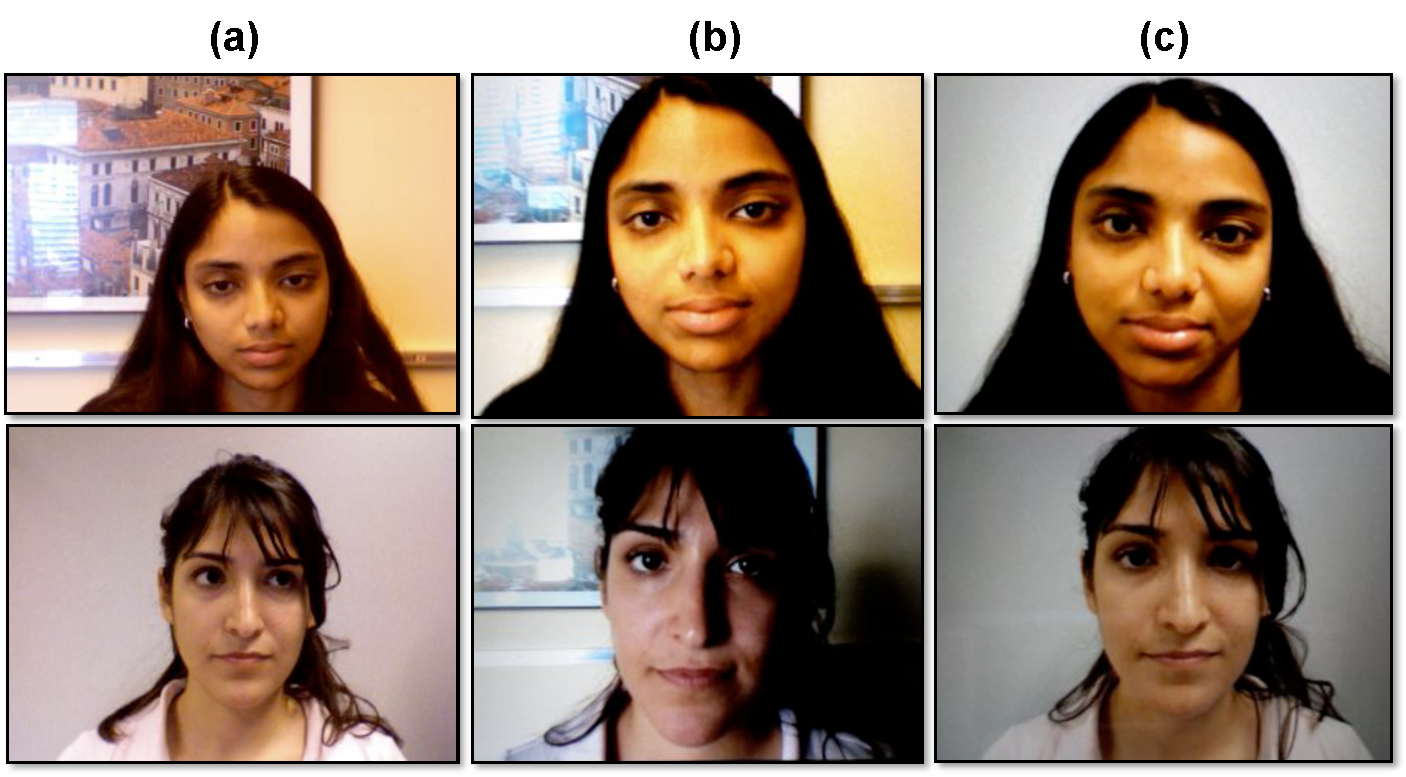
\includegraphics [width=16cm] {images/database_bias.pdf}
\caption[Examples of bias in the Replay Attack Database]{Examples of bias in the Replay Attack Database (a) Real access (b),(c) Attempt of attacks} 
\label{fig:database_bias}
\end{center}
\end{figure}


\begin{table}[ht!]
\caption{$HTER(\%)$ of the trick countermeasure using only the area of the face bounding box  applying the intra-test ($D_1 = D_2$) protocol.}
\begin{center}
  \begin{tabular}{ | c | c | c  c | }
    \hline

    \textbf{Tune} & \textbf{Test} & \multicolumn{2}{c|}{\textbf{HTER(\%)}} \\ 
     $D_1$ & $D_2$ & \textbf{dev} & \textbf{test}  \\ \hline
    
     Replay & Replay & 24.22 & 19.63  \\ 
     CASIA  & CASIA & 51.13 & 53.09  \\
    \hline
  \end{tabular}
\end{center}
\label{tb:TrickCounter}
\end{table}

It can be observed that for the Replay Attack Database the performance in the development and in the test set is far from a random behavior. This experiment confirm the bias observed in this database. It is not possible to observe the same shortcoming in the CASIA FASD. 

\subsubsection{Attack Bias}

The CASIA FASD have different kind of attacks and different way to execute an attack compared to the Replay Attack Database. Exclusive to the CASIA FASD are the warped photo and the cut photo attacks that have no similar in the Replay Attack Database. Exclusive to the Replay Attack Database are the mobile phone attacks. Additionally, the Replay Attack Database has two different support conditions, the fixed and the hand-held. The CASIA FASD has only the hand-held support. \\ \\


\begin{figure*}[ht]
\begin{center}
\includegraphics [width=5cm] {plots/CROSS-DATABASE/MOTION/roc_replay-machine.pdf} 
\includegraphics [width=5cm] {plots/CROSS-DATABASE/LBPTOP/roc_replay-machine.pdf}
\includegraphics [width=5cm] {plots/CROSS-DATABASE/LBP/roc_replay-machine.pdf}

\includegraphics [width=5cm] {plots/CROSS-DATABASE/MOTION/roc_casia_fasd-machine.pdf} 
\includegraphics [width=5cm] {plots/CROSS-DATABASE/LBPTOP/roc_casia_fasd-machine.pdf}
\includegraphics [width=5cm] {plots/CROSS-DATABASE/LBP/roc_casia_fasd-machine.pdf}

\caption[ROC curves of each countermeasure using the intra-test and the inter-test protocol]{ROC curves of each countermeasure using the intra-test and the inter-test protocol. (a) Correlation with frame differences countermeasure trained and tuned with the Replay Attack Database (b) $LBP-TOP$ countermeasure trained and tuned with the Replay Attack Database (c) $LBP$ countermeasure trained and tuned with the Replay Attack Database (d) Correlation with frame differences countermeasure trained and tuned with the CASIA FASD (e) $LBP-TOP$ countermeasure trained and tuned with the CASIA FASD (f) $LBP$ countermeasure trained and tuned with the CASIA FASD.} 
\label{fig:ROC_cross}
\end{center}
\end{figure*}

In next section, we will focus if the countermeasures are truly biased to databases or can be tuned to overcome the database bias.

\subsection{Combination of Multiple Databases}
\label{sec:combination}

In the previous section, we have shown that, with the chosen countermeasures, it was not possible to get a satisfactory performance in both databases at the same time running the inter-test protocol. If we can not achieve that in tests with databases, what can we say about applying these in a real world scenario? If the databases introduce some bias in the countermeasures due to some particularities of them, we can train each countermeasure with a joint training set combining both databases in order to overcame these biases. Figure \ref{img:joint_training} shows a schematic of this joint training. This is the an intuitive approach to create a more robust countermeasure.

\begin{figure}[!htb]
\begin{center}
\includegraphics [width=10cm] {images/joint_training.pdf}
\caption{Joint training scheme for countermeasures} \label{img:joint_training}
\end{center}
\end{figure}



Table \ref{tb:TrainAllTest} shows the performance for each countermeasure trained with this strategy. %The analysis is supported with the ROC curves presented in Figure \ref{tb:TrainAllTest}.

\begin{table}[ht]
\caption{$HTER(\%)$  of each countermeasure trained with Replay Attack Database and CASIA FASD and test it with each test set of each database.}
\begin{center}
  \begin{tabular}{ | c | c | c  c |}
    \hline

   \multirow{2}{*}{\textbf{Countermeasure}} &  \multirow{2}{*}{\textbf{Test}} & \multicolumn{2}{c|}{\textbf{HTER(\%)}} \\ 
    &&\textbf{dev} & \textbf{test}  \\ \hline
    
    \multirow{2}{*}{Correlation} & Replay  &  \multirow{2}{*}{12.18} & 24.14 \\ 
               & CASIA &  & 43.30  \\ \hline \hline

    \multirow{2}{*}{$LBPTOP_{8,8,8,1,1,1}^{u2}$}  & Replay  & \multirow{2}{*}{14.29} & 10.67 \\
               &  CASIA  & & 42.04  \\ \hline \hline

    \multirow{2}{*}{$LBP_{8,1}^{u2}$}  & Replay  & \multirow{2}{*}{20.45} &19.07 \\
                & CASIA  &  & 45.92 \\
    \hline
  \end{tabular}
\end{center}
\label{tb:TrainAllTest}
\end{table}

Analyzing the performances of this strategy compared with the performance obtained with the inter-set protocol, it can be observed a significant improvement for all three countermeasures. However, comparing with the intra-test protocol, the performance drops drastically. It can be observed that the performance for CASIA FASD degrades more than for the Replay Attack Database suggesting a strong bias for this database. 

The results suggest that this strategy is ineffective using these countermeasures. Additionally, this strategy has one possible drawback. In face of new kinds of attacks or new databases it is necessary to train and tune all the countermeasures again. And this could be time consuming.


%\begin{figure}[ht]
%\begin{center}
%\includegraphics [width=5.5cm] {plots/ALL/MOTION.pdf} 
%\includegraphics [width=5.5cm] {plots/ALL/LBPTOP.pdf}
%\includegraphics [width=5.5cm] {plots/ALL/LBP.pdf}
%\caption{ROC curves of each countermeasure trained with Replay Attack Database and CASIA FASD and test it with each test set of each database. (a) Correlation with frame differences (b) $LBP-TOP$ countermeasure (c) $LBP$ countermeasure} 
%\label{fig:ROC_cross}
%\end{center}
%\end{figure}


\subsection{Score Level Fusion based Framework}
\label{sec:framework}

In order to improve the performance results in comparison with the intra-test protocol and the inter-test protocol, and to mitigate the bias mentioned in Section \ref{tb:InterTest}, we introduce a framework based on score level fusion. 

This framework consists of training each countermeasure to one specific database; each one will generate a score and these scores are fused generating the framework output. The fusion strategy used in this dissertation was a simple sum of normalized scores. Figure \ref{img:fusion_framework} shows a schema of the Score Level Fusion based Framework. In this Figure, the same countermeasure are trained with two different databases and each one generates a score. These scores are fused generating the final score of the Framework. 

Using this strategy, when a new countermeasure need to be added, it is possible to ``plug it" in the framework. This strategy is similar to an antivirus software. An antivirus is robust against different kind of attacks and they have regular updates in  order to become more robust against new threats.

\begin{figure}[!htb]
\begin{center}
\includegraphics [width=12cm] {images/fusion_framework.pdf}
\caption[Score Level Fusion based Framework schema]{Score Level Fusion based Framework schema} \label{img:fusion_framework}
\end{center}
\end{figure}


As a support metric for the framework, we first evaluate the level of independence of the countermeasures trained with different databases in order to ensure its effectiveness in a possible score fusion. \cite{kuncheva2003measures} show that the combination of statistically independent classifiers is recommended for a good performance in a score level fusion. In order to evaluate the dependence of classifiers, they analyzed ten statistics. The methodology presented in that work shows that the $Q-statistic$ is most suitable and we choose that metric to evaluate the statistic dependence of each countermeasure for the Score Level Fusion based Framework. The $Q-statistic$ for two classifiers is defined as follow:

\begin{equation}
\label{eq:Qstatistic}
Q_{R,C} = \frac{N_{11}N_{00} - N_{01}N_{10}}{N_{11}N_{00} +N_{01}N_{10}}
\end{equation}
where $R$ is the countermeasure trained with the Replay Attack Database; $C$ is the countermeasure trained with CASIA FASD; $N_{11}$ is the number of times that the countermeasure trained with the Replay Attack Database hits (i.e. correctly classifies a sample) and the countermeasure trained with the CASIA FASD also hits; $N_{10}$ is the number of times that the countermeasure trained with the Replay Attack Database hits and the countermeasure trained with the CASIA FASD misses; $N_{01}$ is the number of times that the countermeasure trained with the Replay Attack Database misses and the countermeasure trained with the CASIA FASD hits and $N_{00}$ is the number of times that the countermeasure trained with the Replay Attack Database misses and the countermeasure trained with the CASIA FASD also misses. The range of this measure goes from -1 to 1.

For statistically independent countermeasures it is expected a $Q_{R,C}$ close to 0. Results close to 1 means that both countermeasures are very similar and there is no improvement in the fusion. Results close -1 indicates that both countermeasures oppose each other and a high degradation in the fusion should be expected. 

Table \ref{tb:FrameworkTest} shows the statistic dependency using the $Q-statistic$ and the performance in each database trained with the Score Level Fusion based Framework. The analysis is supported with the ROC curves presented in Figure \ref{fig:ROC_framework}.

\begin{table}[ht]
\caption{$Q-statistic$ and $HTER(\%)$ of each countermeasure trained with the Score Level Fusion based Framework and test it with each database.}
\begin{center}
  \begin{tabular}{ | c | c | c | c  c |}
    \hline

   \multirow{2}{*}{\textbf{Countermeasure}} &  \multirow{2}{*}{\textbf{Test}} & \multirow{2}{*}{\textbf{$Q_{R,C}$}} & \multicolumn{2}{c|}{\textbf{HTER(\%)}}  \\ 
     &  &  & \textbf{dev} & \textbf{test}  \\ \hline
    
    \multirow{2}{*}{Correlation} & Replay & 0.11 &  \multirow{2}{*}{13.71} & 12.39\\
               & CASIA & -0.14 &  & 32.08 \\ \hline \hline

    \multirow{2}{*}{$LBPTOP_{8,8,8,1,1,1}^{u2}$}  & Replay  & 0.24 &\multirow{2}{*}{23.16} & 26.04 \\
               &  CASIA  & -0.41 & & 38.18 \\ \hline \hline

    \multirow{2}{*}{$LBP_{8,1}^{u2}$}  & Replay  & 0.38 & \multirow{2}{*}{19.69} & 21.66  \\
                & CASIA & -0.41 &  & 47.16 \\
    \hline
  \end{tabular}
\end{center}
\label{tb:FrameworkTest}
\end{table}



\begin{figure*}[ht]
\begin{center}

\includegraphics [width=5.5cm] {plots/FRAMEWORK/MOTION/SUM.pdf} 
\includegraphics [width=5.5cm] {plots/FRAMEWORK/LBPTOP/SUM.pdf}
\includegraphics [width=5.5cm] {plots/FRAMEWORK/LBP/SUM.pdf}

\caption[ROC curves of each countermeasure trained with the Score Level Fusion based Framework]{ROC curves of each countermeasure trained with the Score Level Fusion based Framework (a) Correlation with frame differences (b) $LBP-TOP$ countermeasure (c) $LBP$ countermeasure.} 
\label{fig:ROC_framework}
\end{center}
\end{figure*}

Analyzing the $Q-statistic$ it is  possible to observe that the Correlation with Frame Differences countermeasure is the most statistically independent and suggests that a score fusion is suitable. This can be attested analysing its performance compared with the inter-test (see Table \ref{tb:InterTest}) and intra-test (see Table \ref{tb:IntraTest}) protocol results. For the inter-test protocol the improvement with the Score Level Fusion based Framework was significative. Comparing with the intra-test protocol the degradation was very low and the countermeasure is able to detect spoofs in both databases with different degrees of success.

However the $Q-statistic$ for the $LBP-TOP$ and the $LBP$ countermeasures present unbalanced values for each database. Specially for the CASIA FASD $Q_{R,C}\simeq-0.4$ suggesting that each one of this two countermeasure trained with different databases oppose each other and are not suitable for the Score Level Fusion based Framework. This can be attested analysing their performances compared with the intra-test protocol results (see Table \ref{tb:IntraTest}). The degradation is still high.

%The authors that designed the $LBP$ and $LBP-TOP$ countermeasures chosen the SVM with the RBF kernel as classifier. In both settings, the final trained machines have $\sim35\%$ of the training data as support vectors, what suggest overfitting in each database. The authors that designed the Correlation with Frame Differences countermeasure chosen MLPs with only 5 neurons, which is much simpler classifier and has less chance to overfit of the training data than a SVM.

It is important to remark that the literature lacks in video face spoofing databases and is not possible to ensure the effectiveness of the Score Level Fusion based Framework in a third database. Its effectiveness in a third video face spoofing database, at this stage is only speculative. Another point to highlight is that the fusion strategy chosen for this work is quite simple. For a future extensions more complex fusion strategies need to be addressed.

\section{Final Remarks}
\label{sec:Experiments_finalremarks}

This chapter compared four countermeasures, representing the state of the art of the research field, using two different test protocols. Using the only two video face antispoofing databases publicly currently available (Replay Attack Database and CASIA FASD) we introduced the intra-test protocol and the inter-test protocol.

The evaluation of each countermeasure using the intra-test protocol suggests a good performance and good intra-database generalization power for three countermeasures (Textures with $LBP$, Dynamic textures with $LBP-TOP$  and Motion Correlation). The exception was the countermeasure based on eye blinks. Due to some particularities of the databases, this countermeasure was not effective in this protocol and it was discarded. Using the inter-test protocol, the countermeasures accumulates a lot of degradation suggesting a strong bias in the databases. It was highlighted to kinds of database bias, the capture bias and the attack bias.

To overcame these biases, we introduced two approaches. The first one, combination of multiple databases, combines the train set of each database to train each one of the presented countermeasures. Compared with the inter-test protocol, this strategy improved the countermeasures performance. However, it was observed a strong bias on the Replay Attack Database degrading the performance in the CASIA FASD compared with the intra-test protocol. In the second approach, we introduced the Score Level Fusion based Framework that merges the scores of countermeasures trained with different databases. Only countermeasures that are statistically independent are suitable for an effective score fusion. Analyzing the $Q-statistic$ measure, the Correlation with Frame Differences countermeasure is the most statistically independent and it is the most suitable for the Framework. This was attested comparing the performance of this countermeasure with the performance obtained with the inter-test and intra-test protocols.  However, the framework performance using the $LBP-TOP$ and $LBP$ presented unbalanced values for each database and high absolute values for the $Q-statistic$. This behavior indicated the ``improperness" of fusion for these countermeasures. The results presented in this chapter is reproducible. The source code with instructions on how to reproduce the results is freely available\footnote{\url{https://pypi.python.org/pypi/antispoofing.crossdatabase/}}.

The Score Level Fusion based Framework can be extended to assume different configurations. For example, it is possible to train different countermeasures with a specific kind of attack. Assuming this configuration, each element of the framework will be specialized to solve one problem (video attacks, mask attacks, printed paper, and so on).
Additionally, it is possible to configure the framework to work with different algorithms. For example, it is possible to fuse the scores of the Motion Correlation with the scores of $LBP-TOP$. It is possible even to provide the score of a face verification as an input for the framework. These different configurations are left to be treated in a future work.



\chapter{Conclusions}
\label{chap:Conclusions}

Focusing in antispoofing countermeasures for face authentication, the goal of this masters dissertation is two fold. The first one, we introduce a novel method to detect face spoofing using the spatiotemporal (dynamic texture) extensions of the Local Binary Pattern. The key idea of the approach is to learn and detect the structure and the dynamics of the facial micro-textures that characterise real faces but not fake ones. The second one, is to provide a comparative study of the state of the art countermeasures for face antispoofing. The key contribution of this comparative study is to covers tests in all video face antispoofing databases freely available focusing in the biases that these databases can introduce in the countermeasures.


As emphasized in the beginning, this masters dissertation focuses in a comparative study of antispoofing countermeasures for face authentication. 

The Chapter 

The intra-test protocol enabled us to measure the performance and evaluate the intra-database generalization of countermeasures. The evaluation of each countermeasure using this protocol, suggests that they are effective to detect spoofs in both databases. Even presenting different performances for different databases, the evaluated countermeasures presented a generalization capability. The only exception was the countermeasures based on eye blinks. With one eye blink, as a liveness check, this countermeasure was easy to deceive it, with a $FAR higher than 90\%$. Increasing the number of eye blinks the $FRR$ was higher than 90\%.

The inter-test protocol enabled us to evaluate the inter-database generalization of countermeasures. Using this protocol, was observed that the evaluated countermeasures accumulates a lot of bias from the databases. It was not possible to detect attacks from one database training the countermeasures with another database. It was observed two kinds of database bias. The first one, called \textbf{capture bias}, is a bias related to process of the databases construction. Both databases present different ways to carry out the attacks. The second one, called \textbf{attack bias}, is a bias related to the attacks. There are some attacks exclusive to the CASIA FASD and there are some exclusive to the Replay Attack Database.

In order to overcame these biases we introduce two approaches. The first one, combination of multiple databases, combines the train set of each database to train each one of the presented countermeasures. These strategy brought some improvement in performance, in HTER terms, compared with the both protocols, but the database bias still remains. In the second approach, we introduced the Score Level Fusion based Framework that merges the scores of countermeasures trained with different databases. The results obtained with the Score Level Fusion based Framework suggest that combining two good and not correlated countermeasures leads to significant improvement in performance, in HTER terms, compared with both protocols.


\section{Contributions}

This masters dissertation provided the following contributions:

\begin{enumerate}
	\item A reproducible research, releasing the all source code ....
	\item A promising countermeasure to detect spoof in a video sequences
	\item A method for compare  
\end{enumerate}

\section{Future work}



%As emphasized in the beginning, this master thesis was aimed at improving current face recognition performance rates by investigating the potential advantages of three different subjects related to this research field.

%As future work we will test more complex strategies of score fusion in order to improve the performance results. This Framework is flexible to aggregate not only data from different databases, but can support any kind of configuration. For example it is possible to aggregate countermeasures trained for a specific kind of attack (print attack, video attack, mobile phone attack and so on). Different configurations for the framework will be tested in the future.

\include{Future_Work}
%\appendix{Related Publications}
\begin{appendices}
\chapter{Texture Description with Local Binary Patterns}
\label{AppendixA}

The Local Binary Pattern (LBP) texture descriptor \cite{ojala1996comparative}, is computed in a pixel level basis using a $n \times n$ kernel, thresholding the surroundings of each pixel with the central pixel value and considering the result as a binary value. The decimal form of the LBP code is expressed as:

\begin{equation}
LBP(x_{c},y_{c})=\displaystyle\sum\limits_{n=0}^{N-1} \emph{f}(i_{n}-i_{c})2^n,
\label{eq:LBP}
\end{equation}

\noindent where $i_{c}$ corresponds to the gray intensity of the center pixel ($x_{c}, y_{c}$), $N$ is the number of sampling points, $i_{n}$ is the gray intensity of the n-th surrounding pixel, and $f(x)$ is defined as follows:

\begin{equation}
f(x)  =
\left\lbrace \begin{array}{ccc}
0 & \mbox{if} & x<0 \\
1 & \mbox{if} & x\geq0 
\end{array}. \right.
\label{eq:fx}
\end{equation}

Later, Ojala et al. \cite{ojala2002multiresolution} extended this operator to support surrounding points and radius of a pixel neighbourhood with different shapes and sizes, enabling handling textures at different scales. Fig. \ref{fig_lbpOperator} illustrates the operator calculation and the points distribution in a circular neighbourhood with radius 2, where the pixel values are bilinearly interpolated whenever the sampling point is not in the center of a pixel.

\begin{figure}
\begin{center}
\includegraphics [width=7.5cm] {images/lbp_operator}
\caption{LBP operator. (a) and (b) The basic LBP operator, where the neighbourhood of each pixel is thresholded and a binary number is obtained. (c) A circular neighbourhood example (with 8 neighbour points and radius 2). The pixel values are bilinearly interpolated whenever the sampling point is not in the center of a pixel.} \label{fig_lbpOperator}
\end{center}
\end{figure}

Another important extension proposed by Ojala et al. \cite{ojala2002multiresolution} was the uniform patterns concept ($u2$). A LBP operator is considered uniform if it contains at most two bitwise transitions 0-1 or 1-0 when viewed as a circular bits chain, and according to Ojala et al. \cite{ojala2002multiresolution}, nearly 90 percent of LBP operators observed in images are uniform. In spacial terms, uniform patterns represent some patterns of a texture: spot, flat, area, edge and corner. With an 8-bit representation, there are 58 patterns with at most two bitwise transitions. Fig. \ref{fig_uniformPattern}, extracted from \cite{Chan2008}, describes all possible uniform patterns with 8 neighbours.

\begin{figure}
\begin{center}
\includegraphics [width=12cm] {images/fig_uniformPattern} 
\end{center}
   \caption[All uniform patterns for LBP with 8 neighbours]{All uniform patterns for LBP with 8 neighbours \cite{Chan2008}.}   
\label{fig_uniformPattern}
\end{figure}

Ahonen et al. (see \cite{ahonen2004face} and \cite{ahonen2006face}) adopt the following notation for the LBP operator: $LBP_{P,R}^{u2}$, where the subscript represents the neighbourhood configuration with $P$ sampling points on a circle of radius $R$, and the superscript $u2$ stands for using only uniform patterns and labelling all non-uniform patterns with a single label.

Recently, LBP have been applied to represent face images, yielding in promising results \cite{ahonen2004face}. The face description using LBP consists in computing a histogram of LBP operators, and good results have been achieved using a configuration with 8 circular surrounding pixels and radius 2 (see \cite{ahonen2004face}, \cite{ahonen2006face} and \cite{Rodriguez06}). The LBP histogram-based approach for face description also takes advantage of the LBP operator extensions. As an example, when uniform patterns are used, the number of histogram bins is greatly reduced, since all non-uniform patterns are grouped into a single bin.

A relevant modification in the original LBP operator for face representation is the idea of splitting the face image in small blocks (which can be overlapped or not) and computing the LBP histogram for each block individually, thereby retaining spatial information. So, the face image is described in three different levels: a pixel level, with the calculation of each operator individually; the regional level, with the calculation of histograms for each block; and a global level, with the concatenation of all block histograms \cite{Rodriguez06}. Fig. \ref{fig_lbpDescription} shows all three levels of face description.


\chapter{Related Publications}
\label{AppendixB}


\end{appendices}


%=============================== Bibliografia ===============================================
\addcontentsline{toc}{chapter}{References}
\renewcommand{\bibname}{Bibliografia}
\markboth{Bibliografia}{Bibliografia}

\bibliographystyle{dcu}
\bibliography{meubib}


\end{document}
